\documentclass[a4paper]{article}
\usepackage{hyperref, graphicx, color, alltt, a4wide}
\usepackage{Sweave}
\usepackage[round]{natbib}
\definecolor{Red}{rgb}{0.7,0,0}
\definecolor{Blue}{rgb}{0,0,0.8}
\definecolor{hellgrau}{rgb}{0.55,0.55,0.55}
\newcommand{\pkg}[1]{{\normalfont\fontseries{b}\selectfont #1}}
\newcommand{\var}[1]{\textit{\texttt{#1}}}
\newcommand{\email}[1]{\href{mailto:#1}{\normalfont\texttt{#1}}}
\newcommand{\data}[1]{`\texttt{#1}'}

%% \code without `-' ligatures
\def\nohyphenation{\hyphenchar\font=-1 \aftergroup\restorehyphenation}
\def\restorehyphenation{\hyphenchar\font=`-}
{\catcode`\-=\active%
  \global\def\code{\bgroup%
    \catcode`\-=\active \let-\codedash%
    \Rd@code}}
\def\codedash{-\discretionary{}{}{}}
\def\Rd@code#1{\texttt{\nohyphenation#1}\egroup}

\newcommand{\codefun}[1]{\code{#1()}}

\begin{document}

%\VignetteIndexEntry{Labeling in the Strucplot Framework}
%\VignetteDepends{vcd}
%\VignetteKeywords{graphics, categorical data}
%\VignettePackage{vcd}


\setkeys{Gin}{width=0.7\textwidth}


\title{Labeling in the Strucplot Framework}
\author{by David Meyer, Achim Zeileis, and Kurt Hornik}
\date{}
\maketitle
\sloppy

\section{Introduction}

One of the major enhancements in package \pkg{vcd} compared to
\codefun{mosaicplot} and \codefun{assocplot} in
base {\sf R} is the labeling in the strucplot framework which 
offers many more features and flexibility. 
Like shading, spacing, and drawing of legend and core plot, 
labeling is now carried out by specialized graphical appearance control
(``grapcon'') functions. This renders labeling completely
modular (see the introductory vignette: ``The Strucplot
Framework---Visualizing Multi-way Contingency Tables'' for an overview).
The user supplies either a labeling function, or, alternatively, 
a generating function that parameterizes a labeling function, 
to \codefun{strucplot} which then draws the labels (the idea behind generating
functions is discussed in detail in the vignette: ``Colors and
Residual-based Shadings in the Strucplot Framework''). 
Labeling is well-separated from the actual plotting that occurs in the
low-level core functions. It only relies on the viewport tree produced by them, and the
`\texttt{dimnames}' attribute of the visualized table. Labeling
functions are grapcons that ``add ink to the canvas'': the drawing of the
labels happens after the actual plot has been drawn by the core function.
Thus, it is possible to supply one's own labeling function, or
to combine some of the basic functions to produce a more complex labeling.
In the following, we describe the three basic modules
(\codefun{labeling\_text}, \codefun{labeling\_list}, and \codefun{labeling\_cells}) and
derived functions that build upon them.

\section{Labels in the borders: \texttt{labeling\_text()}}

\codefun{labeling\_text} is the default for all strucplot displays. It
plots labels in the borders similar to the \codefun{mosaicplot}
function in base {\sf R}, but is much more flexible: it is not limited
to 4 dimensions, and the positioning and graphical parameters 
of levels and variable names are customizable. In addition,
the problem of overlapping labels can be handled in several ways. 

As an example, consider the \data{Titanic} data, consisting
of 4 categorical variables: survival (`survived'), gender (i.e., `sex'), age, and
crew. By default, the variable names and levels are plotted `around' the
plot in a counter-clockwise way (see Figure \ref{fig:defaults}):

\begin{Schunk}
\begin{Sinput}
> mosaic(Titanic)
\end{Sinput}
\end{Schunk}

\begin{figure}[p]
\begin{center}
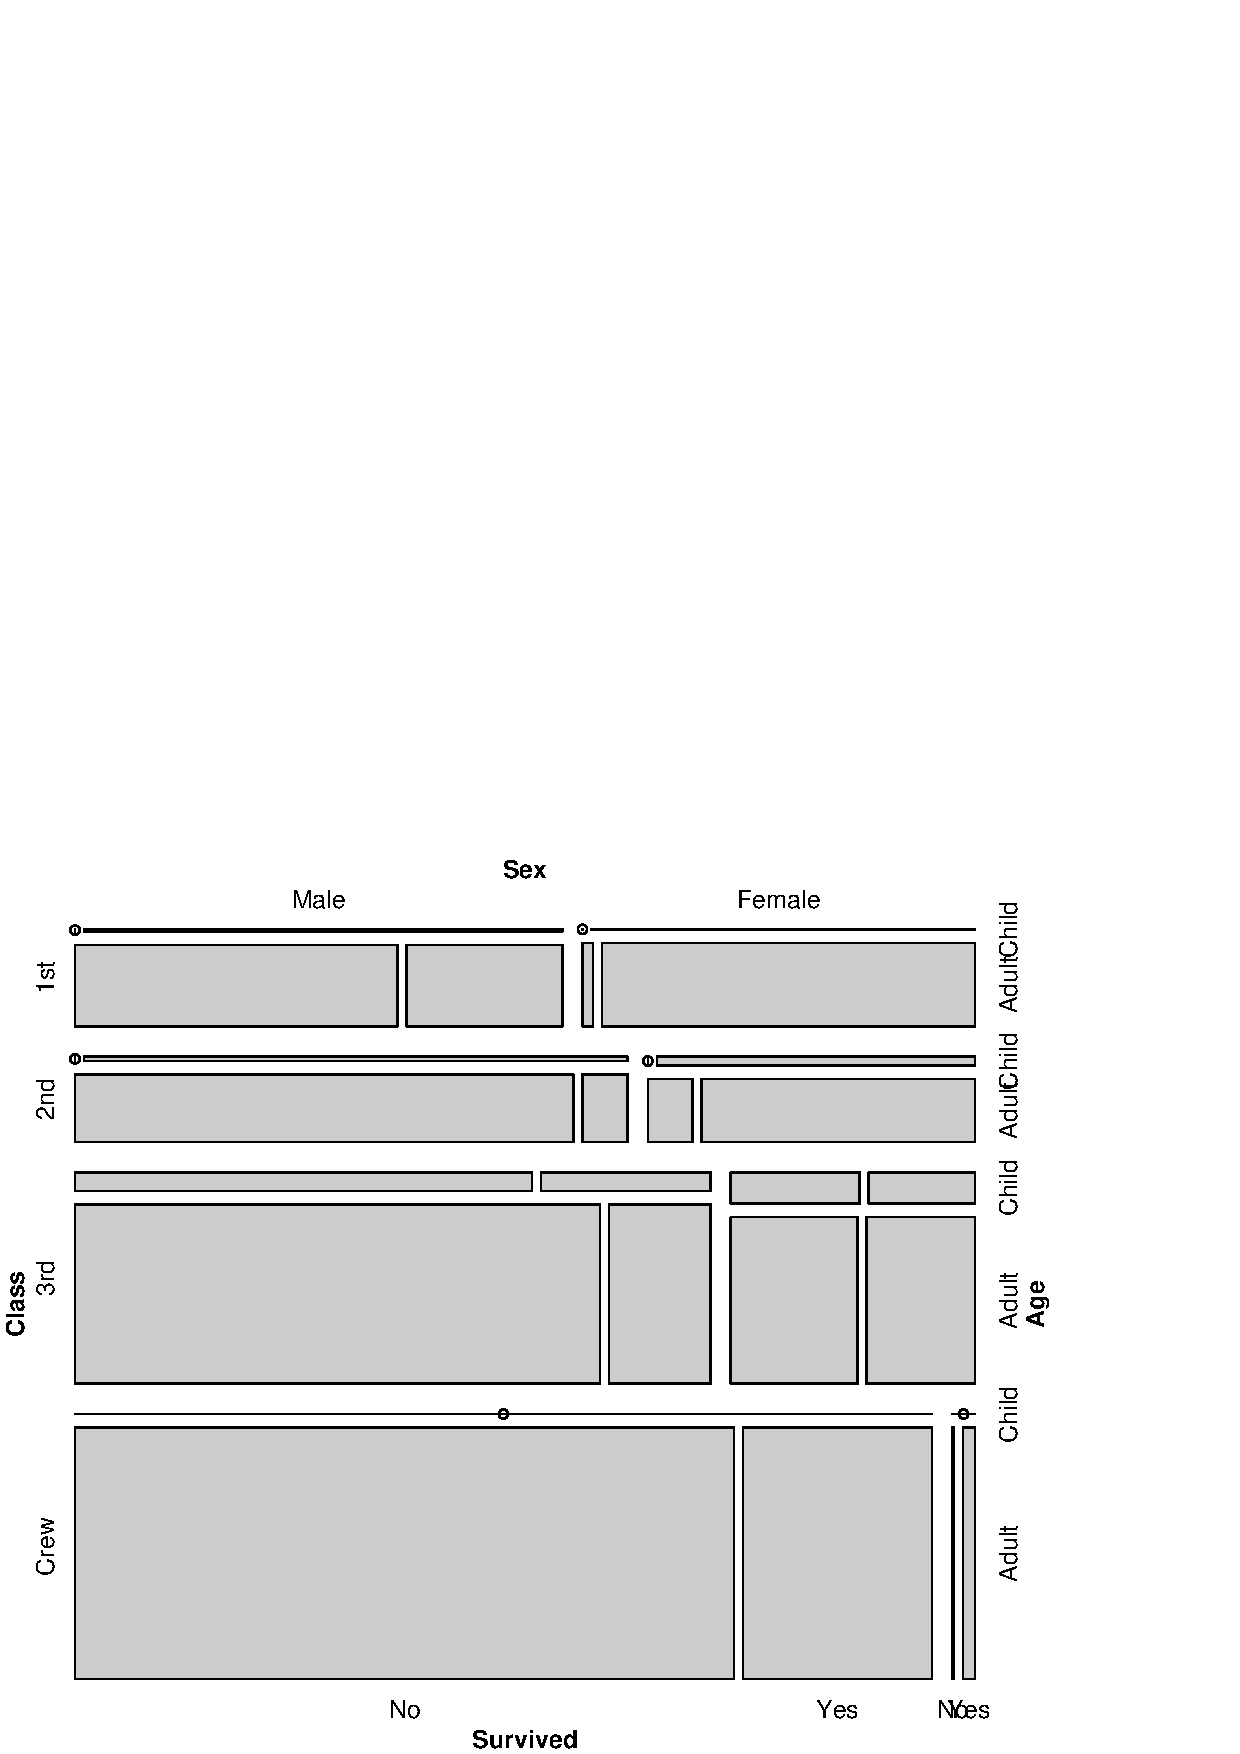
\includegraphics{labeling-defaultfig}
\caption{Mosaic plot for the \data{Titanic} data with default settings
  for labeling.}
\label{fig:defaults}
\end{center}
\end{figure}

\noindent Note that the last two levels of the `survived' variable do
overlap, as well as some adult and child labels of the `age' Variable.
This issue can be addressed in several ways. The `brute force'
method is to enable clipping for these dimensions (see Figure \ref{fig:clipping}):

\begin{Schunk}
\begin{Sinput}
> mosaic(Titanic, labeling_args = list(clip = c(Survived = TRUE, 
+     Age = TRUE)))
\end{Sinput}
\end{Schunk}

\begin{figure}[p]
\begin{center}
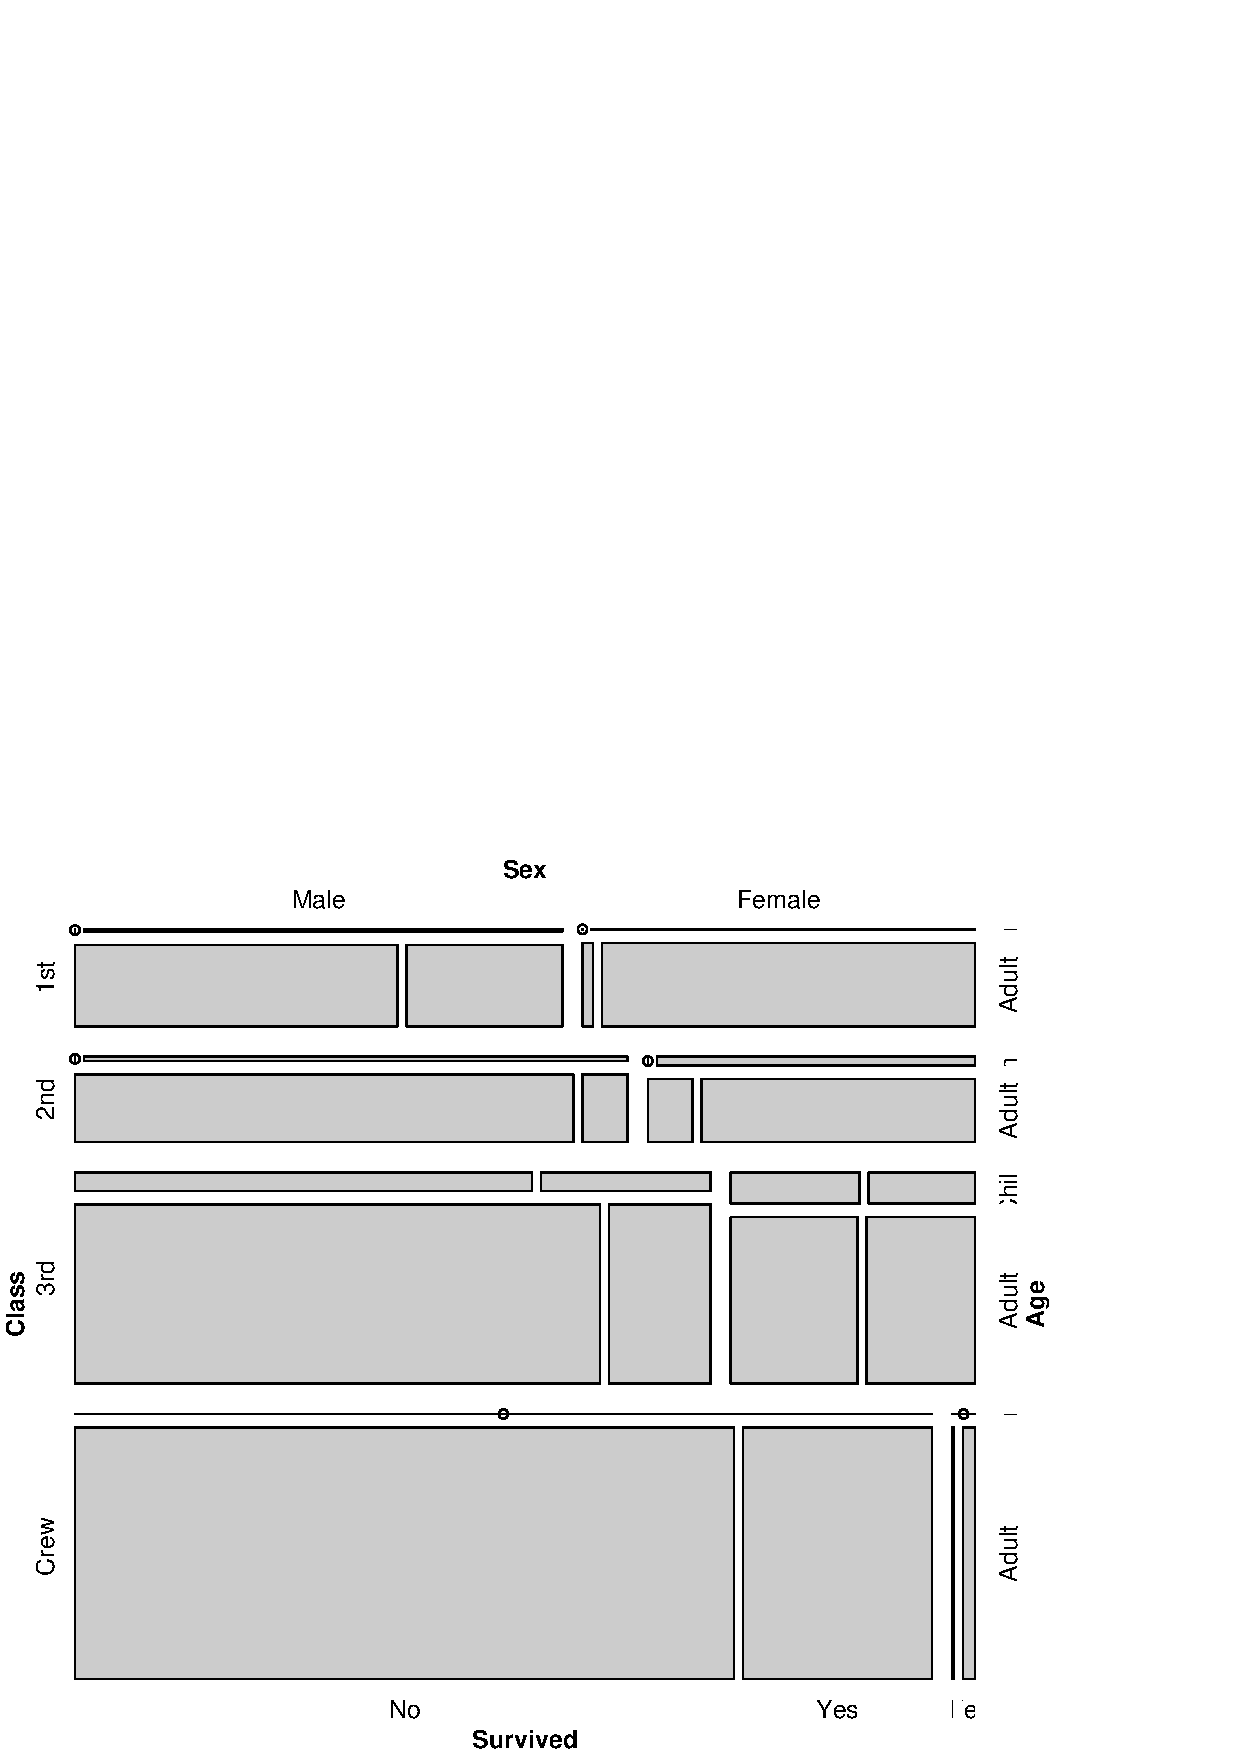
\includegraphics{labeling-clippingfig}
\caption{The effect of clipping.}
\label{fig:clipping}
\end{center}
\end{figure}

\noindent The \code{clip} parameter is passed to the labeling function
via the \code{labeling\_args} argument which takes a list of
parameters. \code{clip} itself takes a vector of logicals (one for
each dimension). 
% as mentioned before
Almost all vectorized arguments in the strucplot
framework can be abbreviated in the following way: unnamed components
(or the defaults, if there are none) are recycled as needed, but
overridden by the named components. Here, the default is \code{FALSE},
and therefore clipping is enabled only for the `survived' and `age' variables.
A more sensible solution to the overlap problem is to abbreviate the 
levels (see Figure \ref{fig:abbreviating}):

\begin{Schunk}
\begin{Sinput}
> mosaic(Titanic, labeling_args = list(abbreviate = c(Survived = TRUE, 
+     Age = 3)))
\end{Sinput}
\end{Schunk}

\begin{figure}[h]
\begin{center}
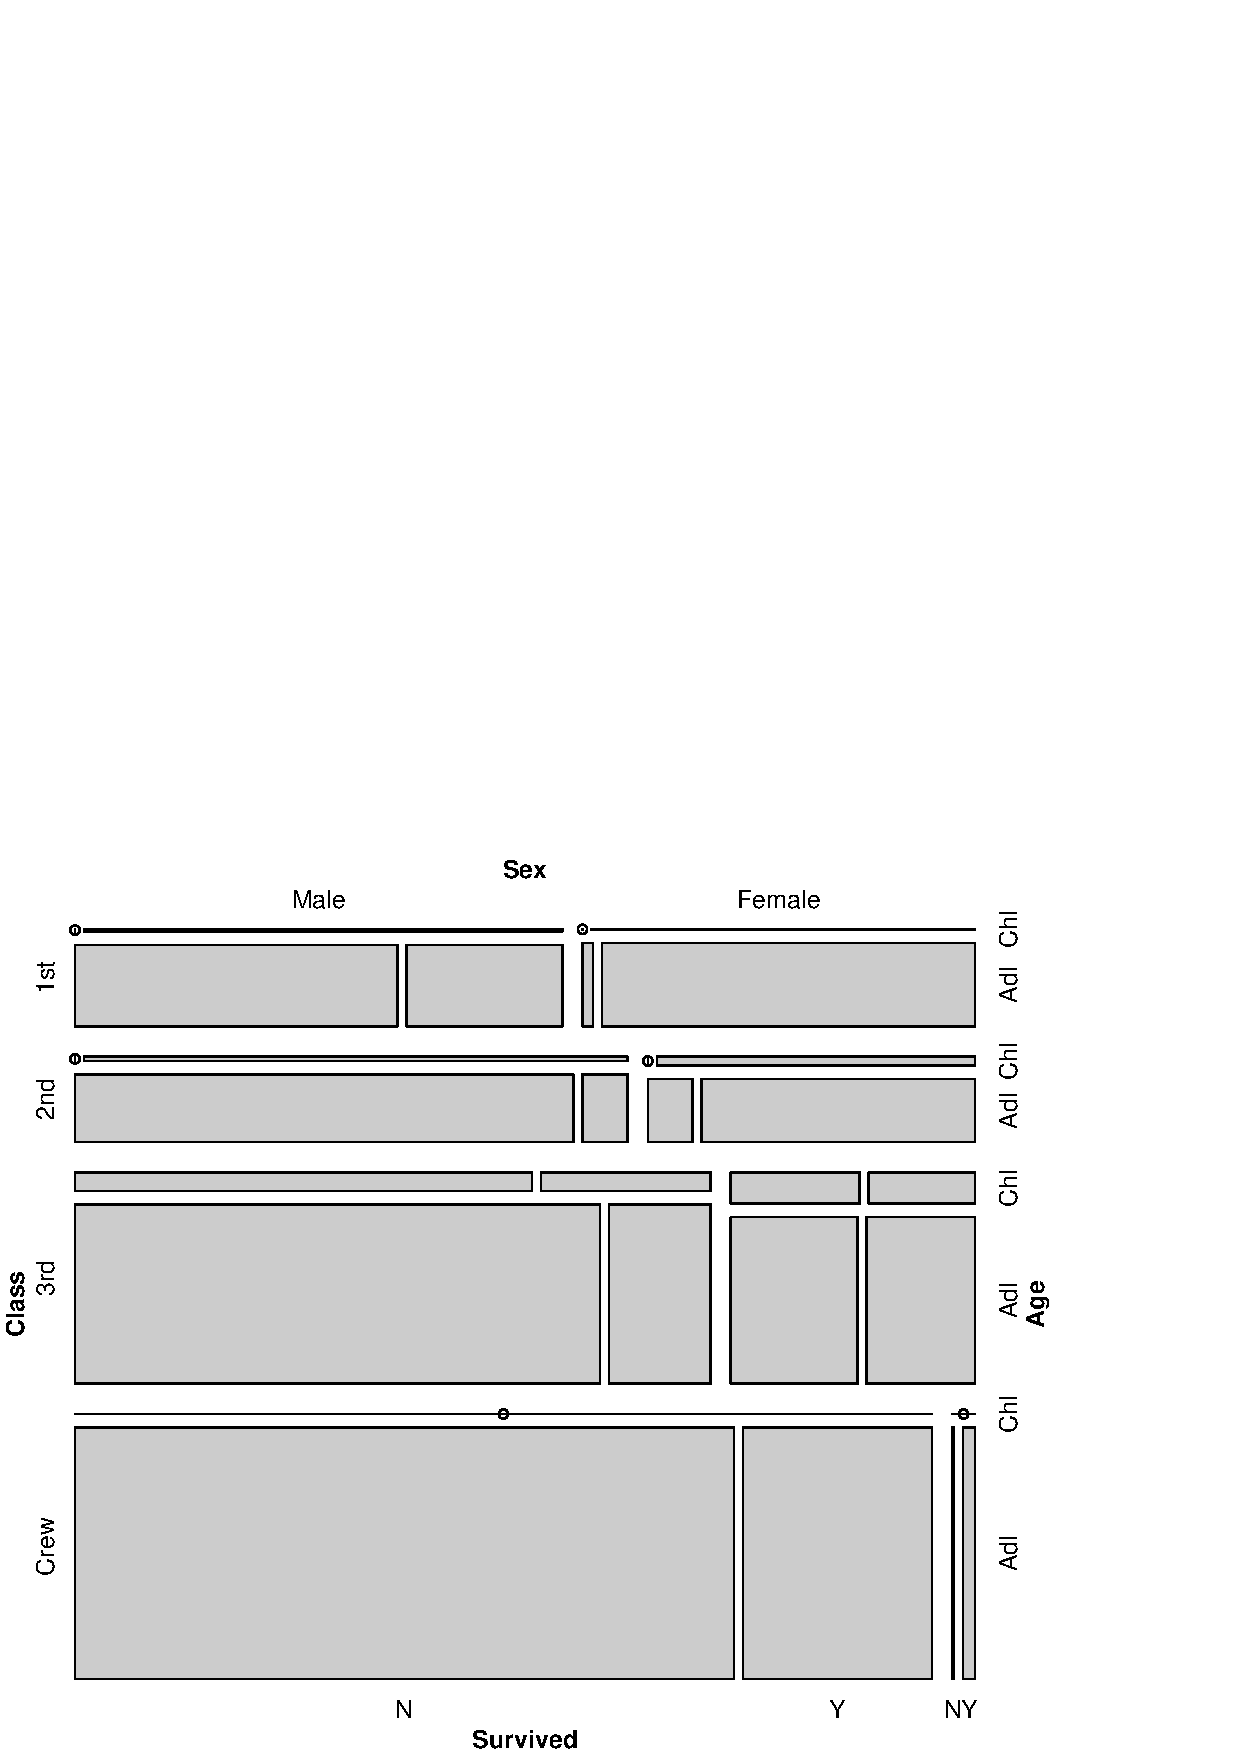
\includegraphics{labeling-abbreviatingfig}
\caption{Abbreviating.}
\label{fig:abbreviating}
\end{center}
\end{figure}

\noindent The \code{abbreviate} argument takes a vector of
integers indicating the number of significant characters the levels should be
abbreviated to (\code{TRUE} is interpreted as 1, obviously). Abbreviation
is performed using the \codefun{abbreviate} function in base {\sf R}. Another
possibility is to rotate the levels (see Figure~\ref{fig:rotating}):

\begin{Schunk}
\begin{Sinput}
> mosaic(Titanic, labeling_args = list(rot_labels = c(bottom = 90, 
+     right = 0), offset_varnames = c(right = 1), offset_labels = c(right = 0.3)), 
+     margins = c(right = 4, bottom = 3))
\end{Sinput}
\end{Schunk}

\begin{figure}[p]
\begin{center}
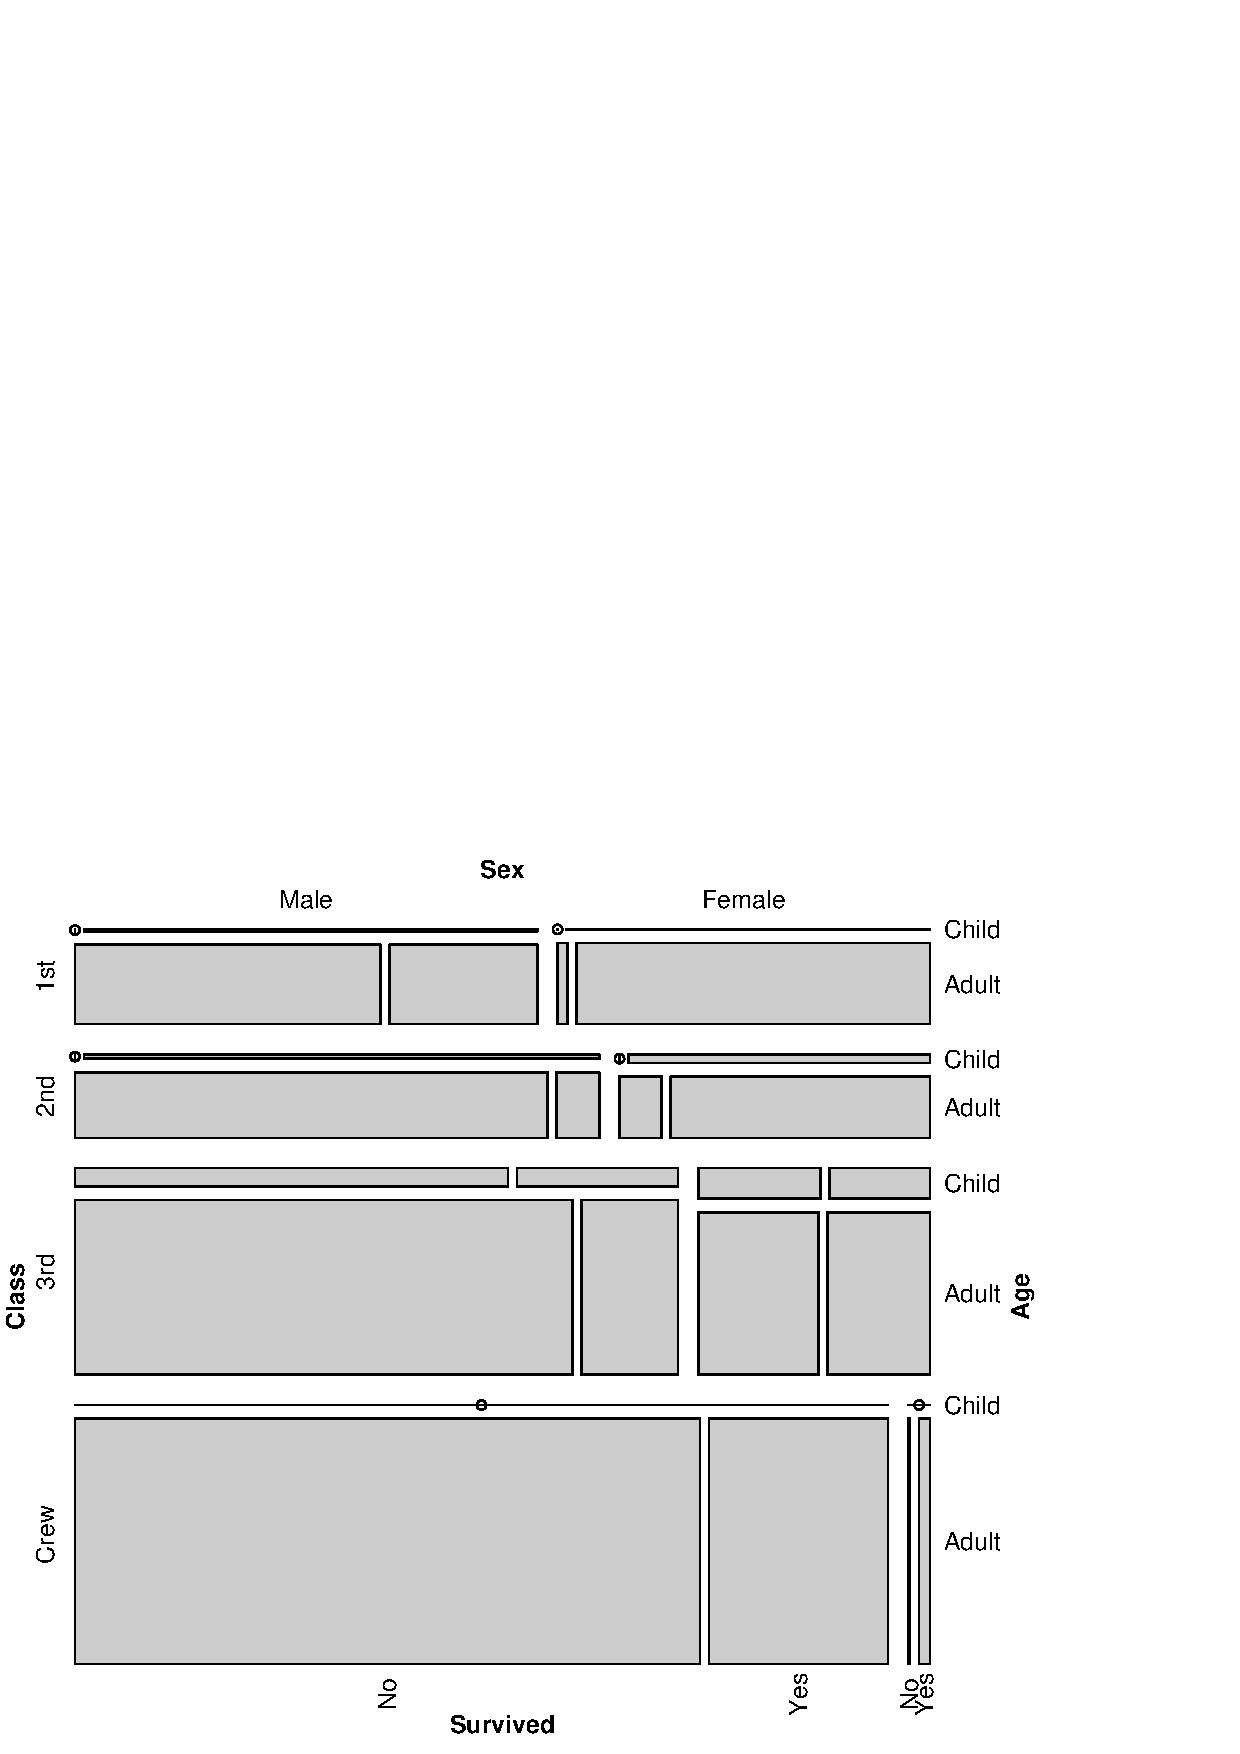
\includegraphics{labeling-rotatefig}
\caption{Rotating labels.}
\label{fig:rotating}
\end{center}
\end{figure}

\noindent Finally, we could also inhibit the output of repeated levels 
(see Figure \ref{fig:repeat}):

\begin{Schunk}
\begin{Sinput}
> mosaic(Titanic, labeling_args = list(rep = c(Survived = FALSE, 
+     Age = FALSE)))
\end{Sinput}
\end{Schunk}

\begin{figure}[p]
\begin{center}
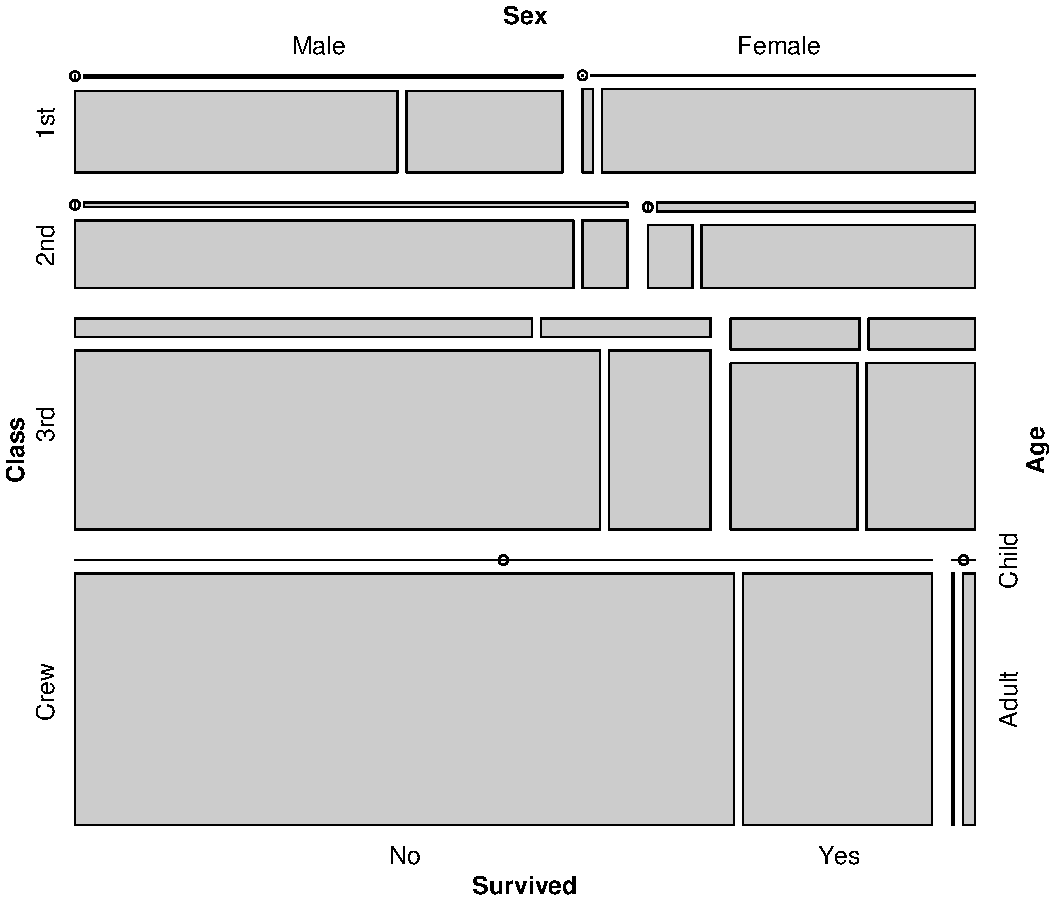
\includegraphics{labeling-repeatfig}
\caption{Inhibiting the repetition of levels.}
\label{fig:repeat}
\end{center}
\end{figure}

We now proceed with a few more `cosmetic' features (which do not all
produce satisfactory results for our sample data).
A first simple, but effectful modification is to position
all labels and variables left-aligned:  (see Figure \ref{fig:left}):

\begin{Schunk}
\begin{Sinput}
> mosaic(Titanic, labeling_args = list(pos_varnames = "left", 
+     pos_labels = "left", just_labels = "left", rep = FALSE))
\end{Sinput}
\end{Schunk}

\begin{figure}[h]
\begin{center}
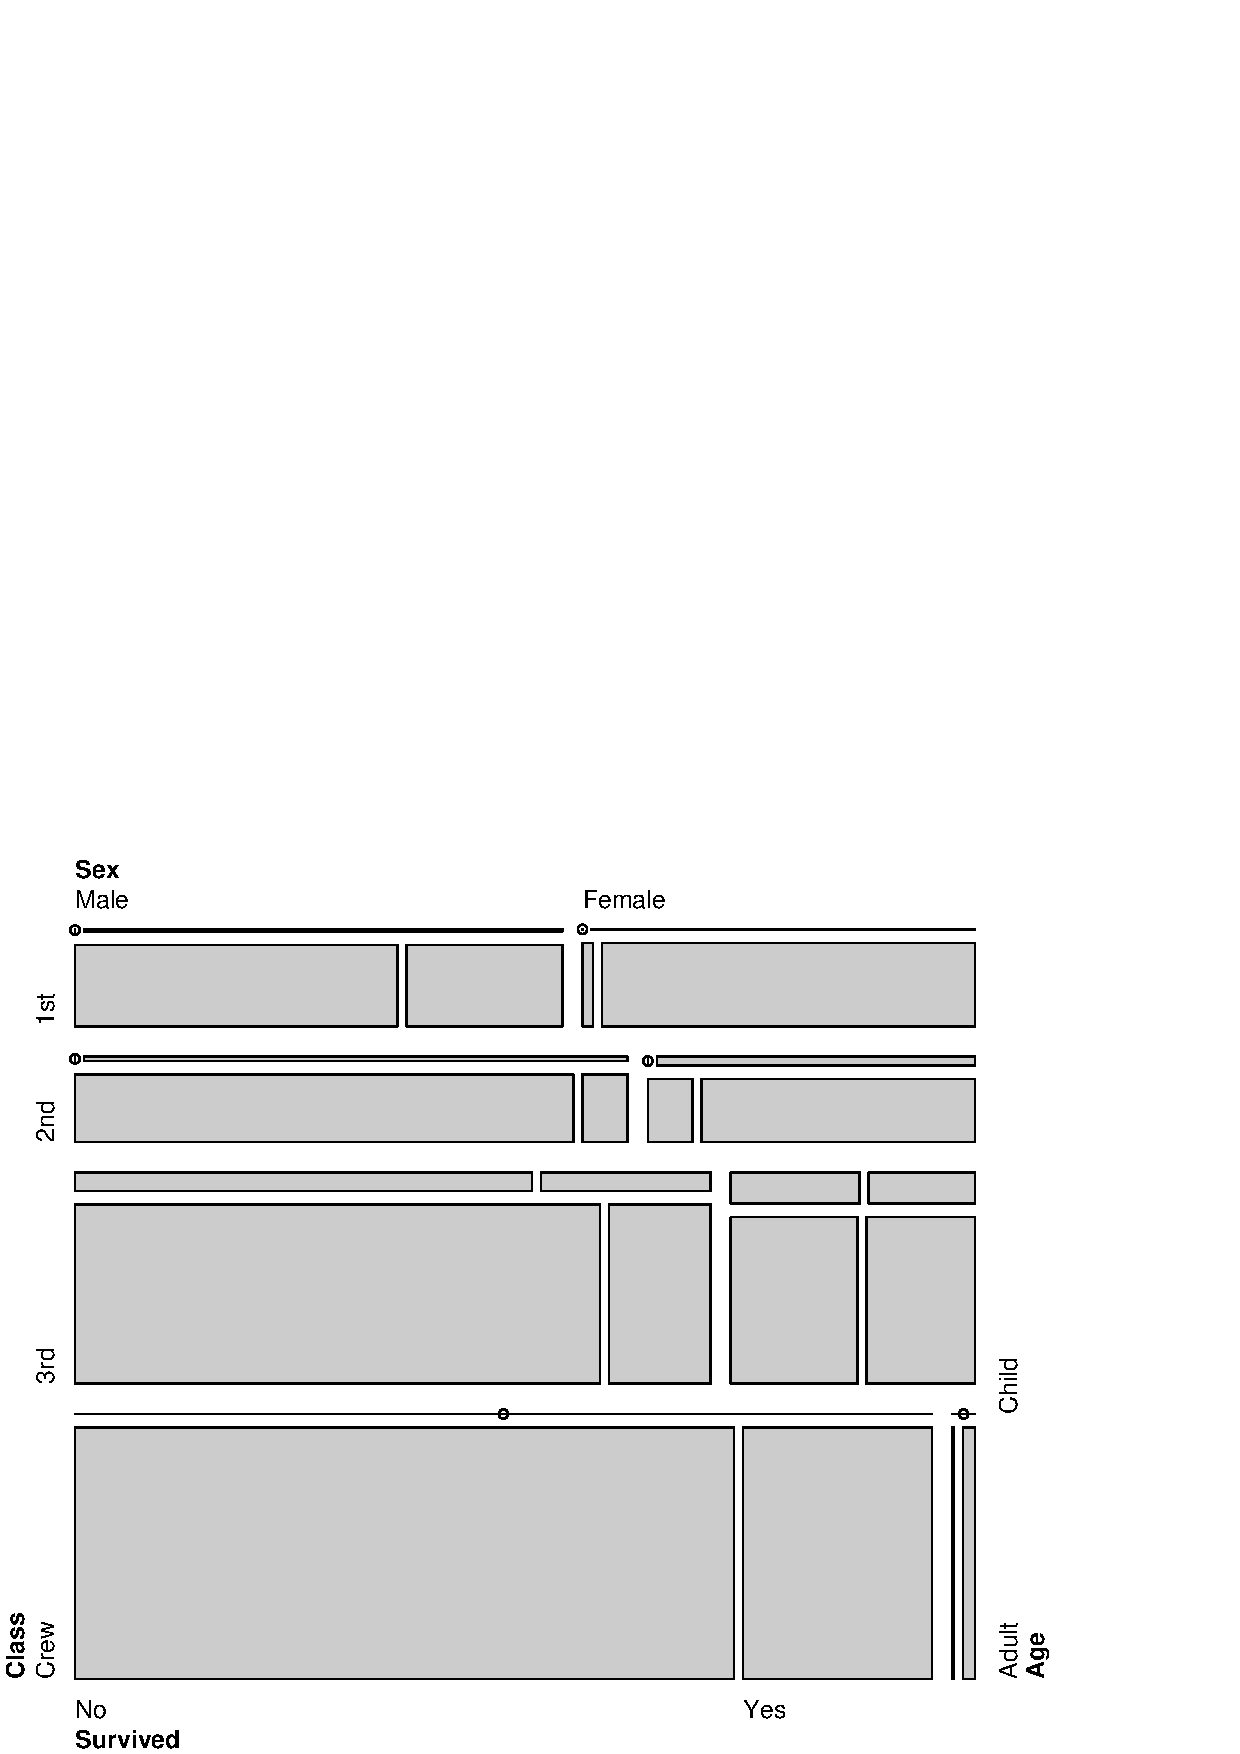
\includegraphics{labeling-leftfig}
\caption{Left-aligning.}
\label{fig:left}
\end{center}
\end{figure}

\noindent Note that obviously we need to change the justification 
to \code{"left"} as well. We can
achieve the same effect by using the convenience function \codefun{labeling\_left}: 

\begin{Schunk}
\begin{Sinput}
> mosaic(Titanic, labeling = labeling_left)
\end{Sinput}
\end{Schunk}

\noindent Next, we show how to put all levels to the
bottom and right margins, and all variable names to the top and left
margins (see Figure \ref{fig:margins}):

\begin{Schunk}
\begin{Sinput}
> mosaic(Titanic, labeling_args = list(tl_labels = FALSE, 
+     tl_varnames = TRUE, abbreviate = c(Survived = 1, 
+         Age = 3)))
\end{Sinput}
\end{Schunk}

\begin{figure}[p]
\begin{center}
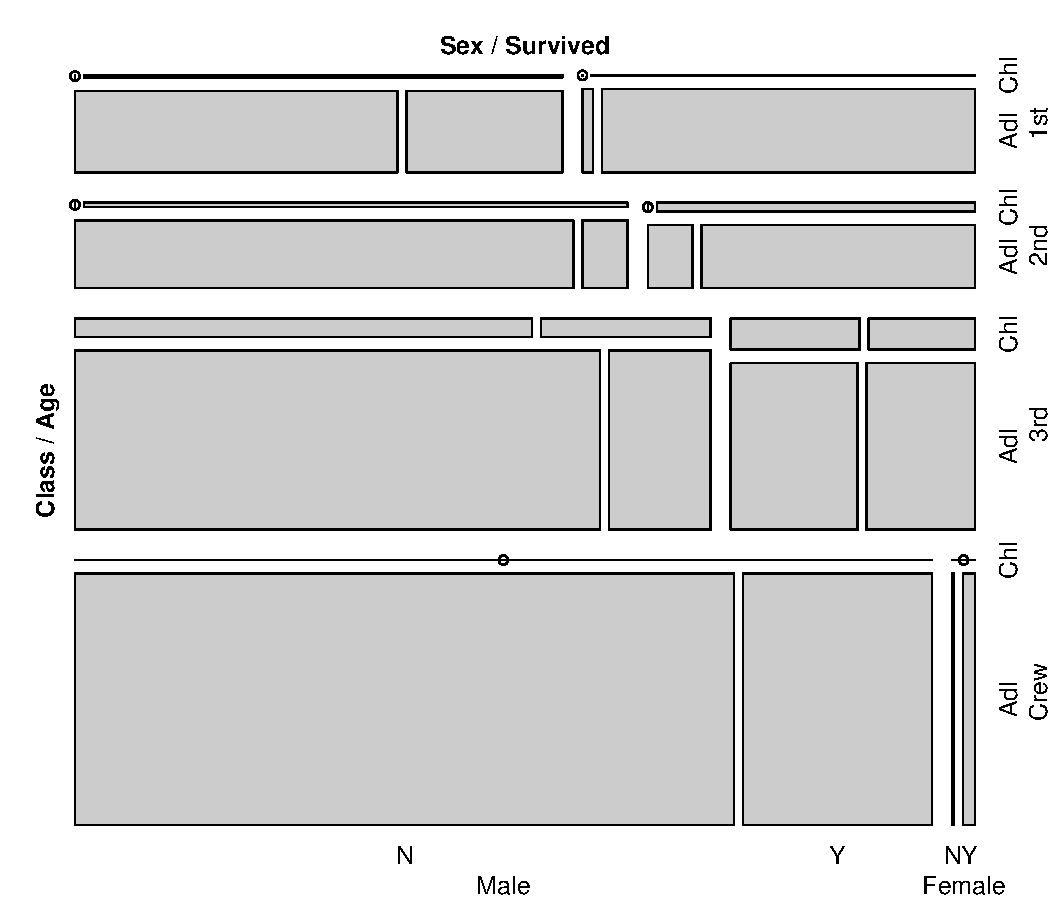
\includegraphics{labeling-marginsfig}
\caption{Changes in the margins.}
\label{fig:margins}
\end{center}
\end{figure}

\noindent The \var{tl\_foo} (``top left'') arguments are \code{TRUE} by default. 
Now, we will add boxes to the labels and additionally
enable clipping (see Figure \ref{fig:boxes}):

\begin{Schunk}
\begin{Sinput}
> mosaic(Titanic, labeling_args = list(tl_labels = FALSE, 
+     tl_varnames = TRUE, boxes = TRUE, clip = TRUE))
\end{Sinput}
\end{Schunk}

\begin{figure}[p]
\begin{center}
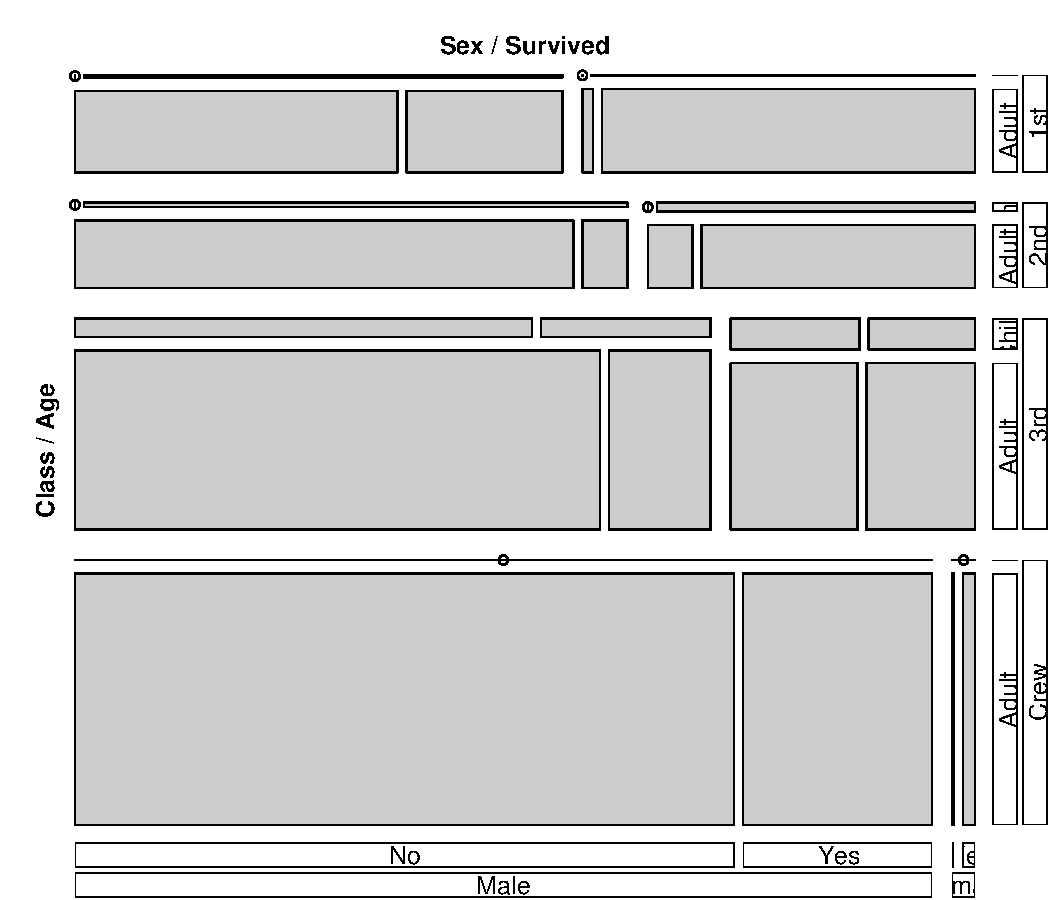
\includegraphics{labeling-boxesfig}
\caption{Boxes and Clipping.}
\label{fig:boxes}
\end{center}
\end{figure}

\noindent The values to \code{boxes} and \code{clip} are recycled for
all dimensions. The result is pretty close to what calling
\codefun{mosaic} with the \codefun{labeling\_cboxed}
wrapper does, except that variables and levels, by default, are put to the top and
to the left of the plot:

\begin{Schunk}
\begin{Sinput}
> mosaic(Titanic, labeling = labeling_cboxed)
\end{Sinput}
\end{Schunk}

\noindent Another variant is to put the variable names into the
same line as the levels (see Figure \ref{fig:labbl}):

\begin{Schunk}
\begin{Sinput}
> mosaic(Titanic, labeling_args = list(tl_labels = TRUE, 
+     boxes = TRUE, clip = c(Survived = FALSE, TRUE), labbl_varnames = TRUE), 
+     margins = c(left = 4, right = 1, 3))
\end{Sinput}
\end{Schunk}

\begin{figure}[h]
\begin{center}
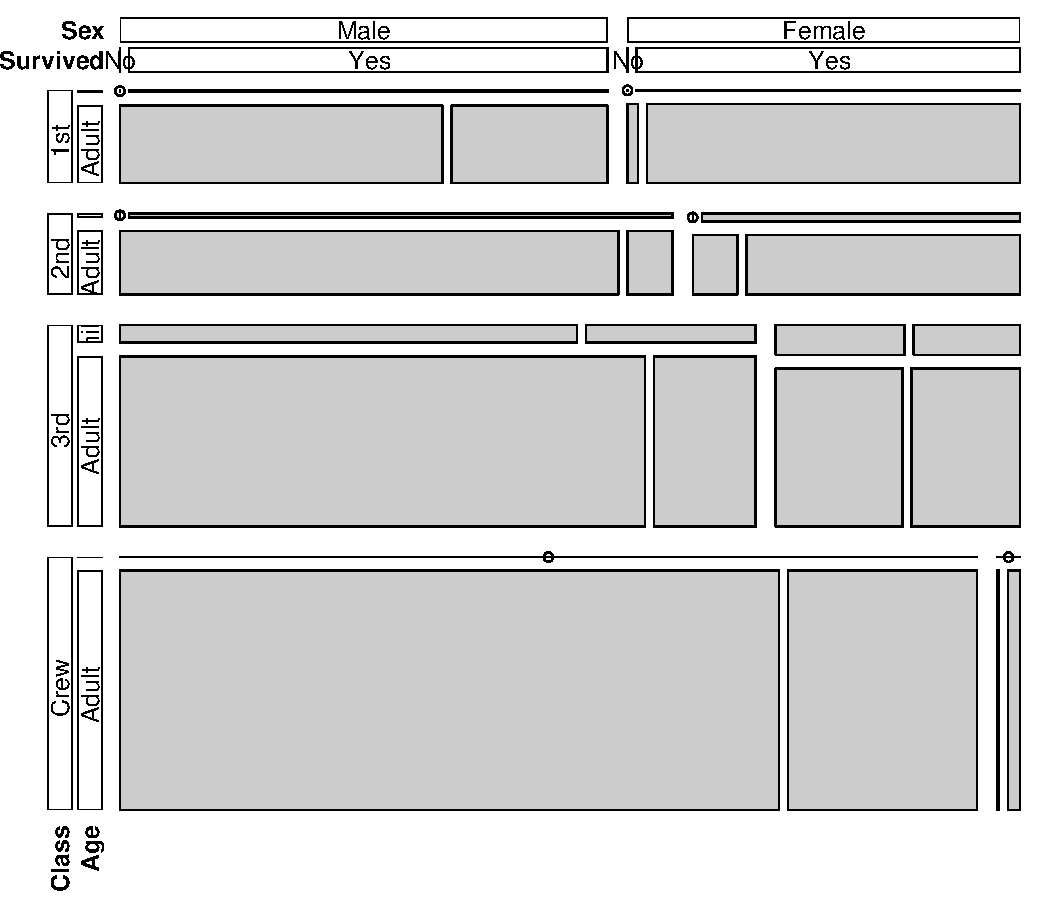
\includegraphics{labeling-labblfig}
\caption{Variable names beneath levels.}
\label{fig:labbl}
\end{center}
\end{figure}

\noindent \code{labbl\_varnames} (``variable names to the bottom/left of the
labels'') is a vector of logicals indicating the side for the
variable names. The resulting layout is close to what
\codefun{labeling\_lboxed} produces, except that variables and levels,
by default, are left-aligned and put to the bottom and to the right of the plot:

\begin{Schunk}
\begin{Sinput}
> mosaic(Titanic, labeling = labeling_lboxed, margins = c(right = 4, 
+     left = 1, 3))
\end{Sinput}
\end{Schunk}

\noindent A similar design is used by the \codefun{doubledecker} function.

\section{Labels in the cells: \texttt{labeling\_cells()}}

This labeling draws both variable names and levels in the
cells. As an example, we use the \data{PreSex} data on pre- and
extramarital sex and divorce (see Figure \ref{fig:cell}):

\begin{Schunk}
\begin{Sinput}
> mosaic(~MaritalStatus + Gender, data = PreSex, labeling = labeling_cells)
\end{Sinput}
\end{Schunk}

\begin{figure}[h]
\begin{center}
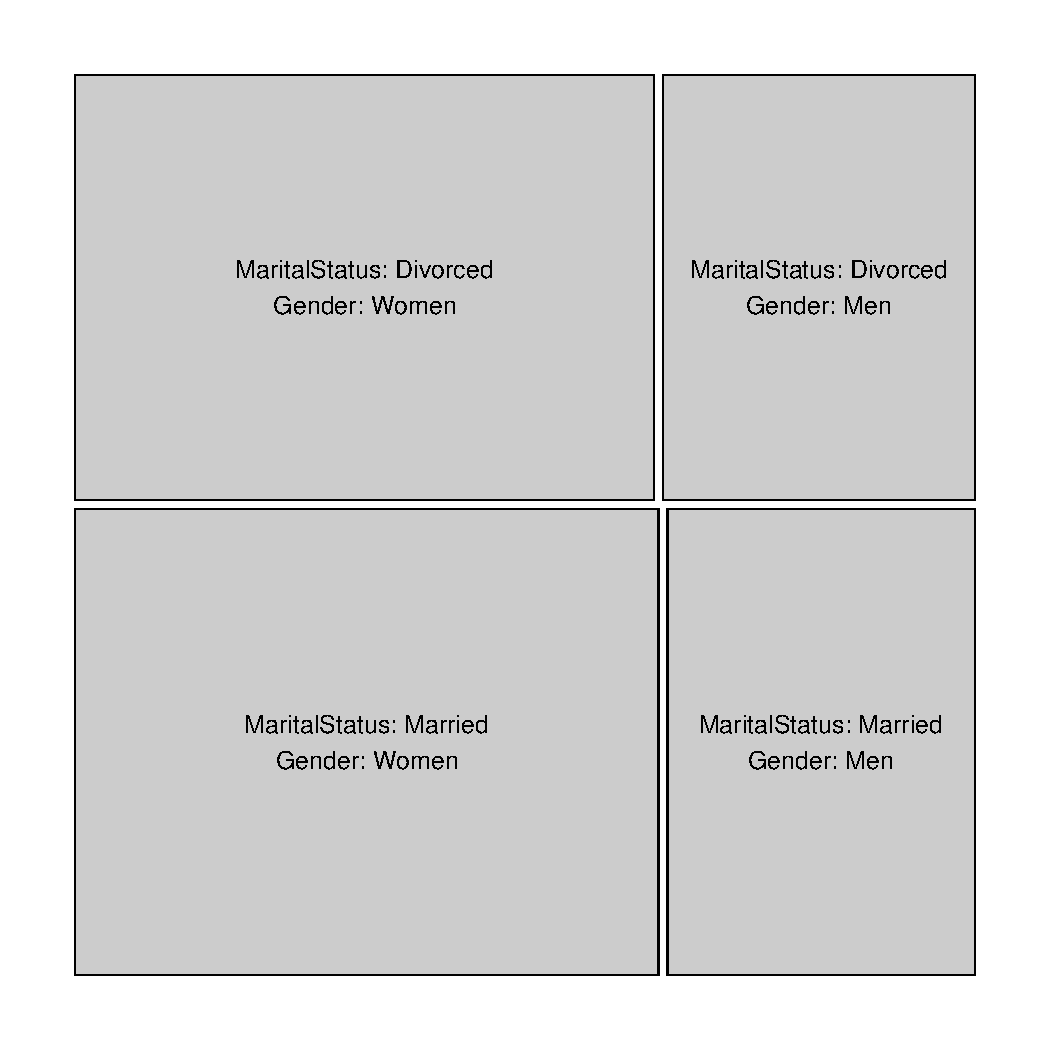
\includegraphics{labeling-cellfig}
\caption{Cell labeling for the \data{PreSex} data.}
\label{fig:cell}
\end{center}
\end{figure}

\noindent In the case of narrow cells, it might be useful to
abbreviate labels and/or variable names and turn off clipping (see Figure \ref{fig:cell2}):

\begin{Schunk}
\begin{Sinput}
> mosaic(~PremaritalSex + ExtramaritalSex, data = PreSex, 
+     labeling = labeling_cells(abbreviate_labels = TRUE, 
+         abbreviate_varnames = TRUE, clip = FALSE))
\end{Sinput}
\end{Schunk}

\begin{figure}[h]
\begin{center}
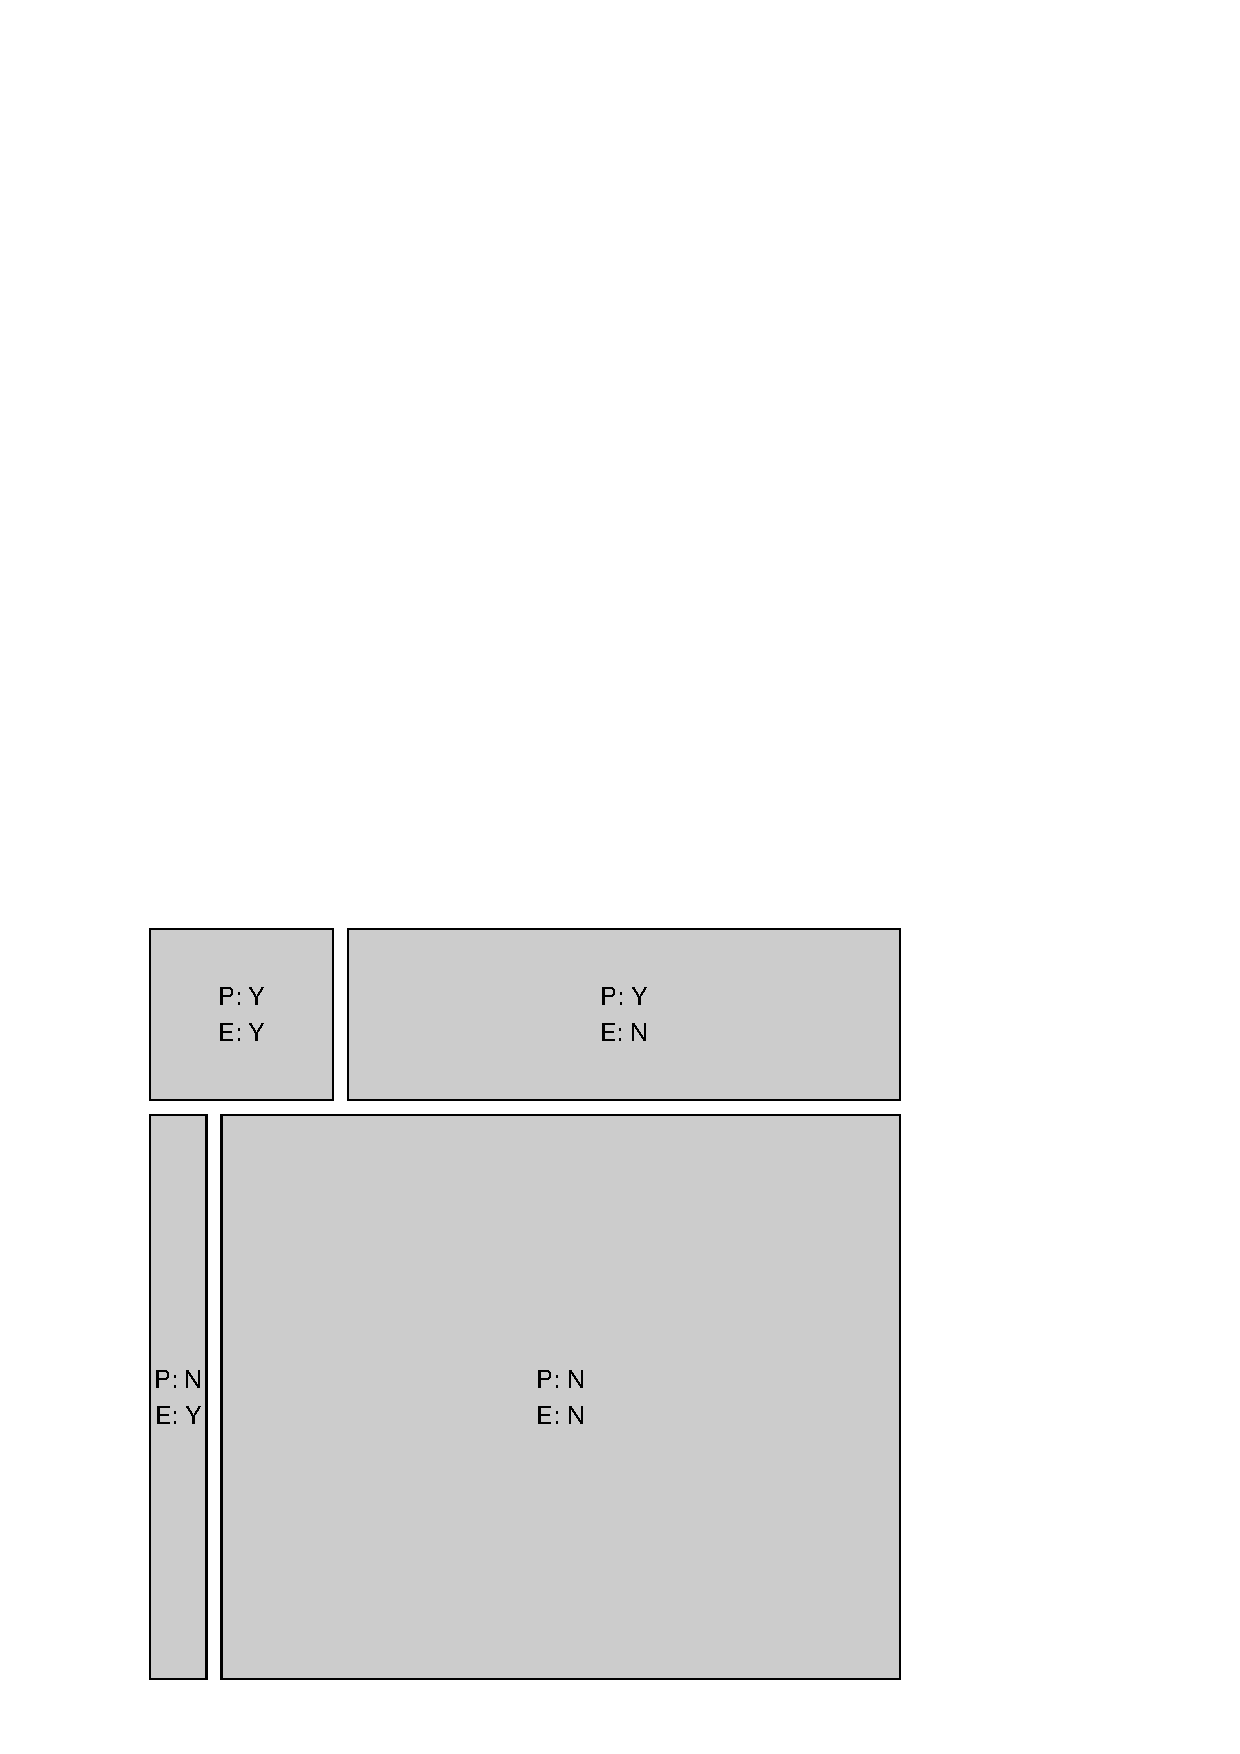
\includegraphics{labeling-cell2fig}
\caption{Cell labeling for the \data{PreSex} data, labels abbreviated.}
\label{fig:cell2}
\end{center}
\end{figure}

\noindent For some data, it might be convenient to combine cell
labeling with border labeling as done by \codefun{labels\_conditional}
(see Figure \ref{fig:conditional}):

\begin{Schunk}
\begin{Sinput}
> mosaic(~PremaritalSex + ExtramaritalSex | MaritalStatus + 
+     Gender, data = PreSex, labeling = labeling_conditional(abbreviate_varnames = TRUE, 
+     abbreviate_labels = TRUE, clip = FALSE))
\end{Sinput}
\end{Schunk}

\begin{figure}[h]
\begin{center}
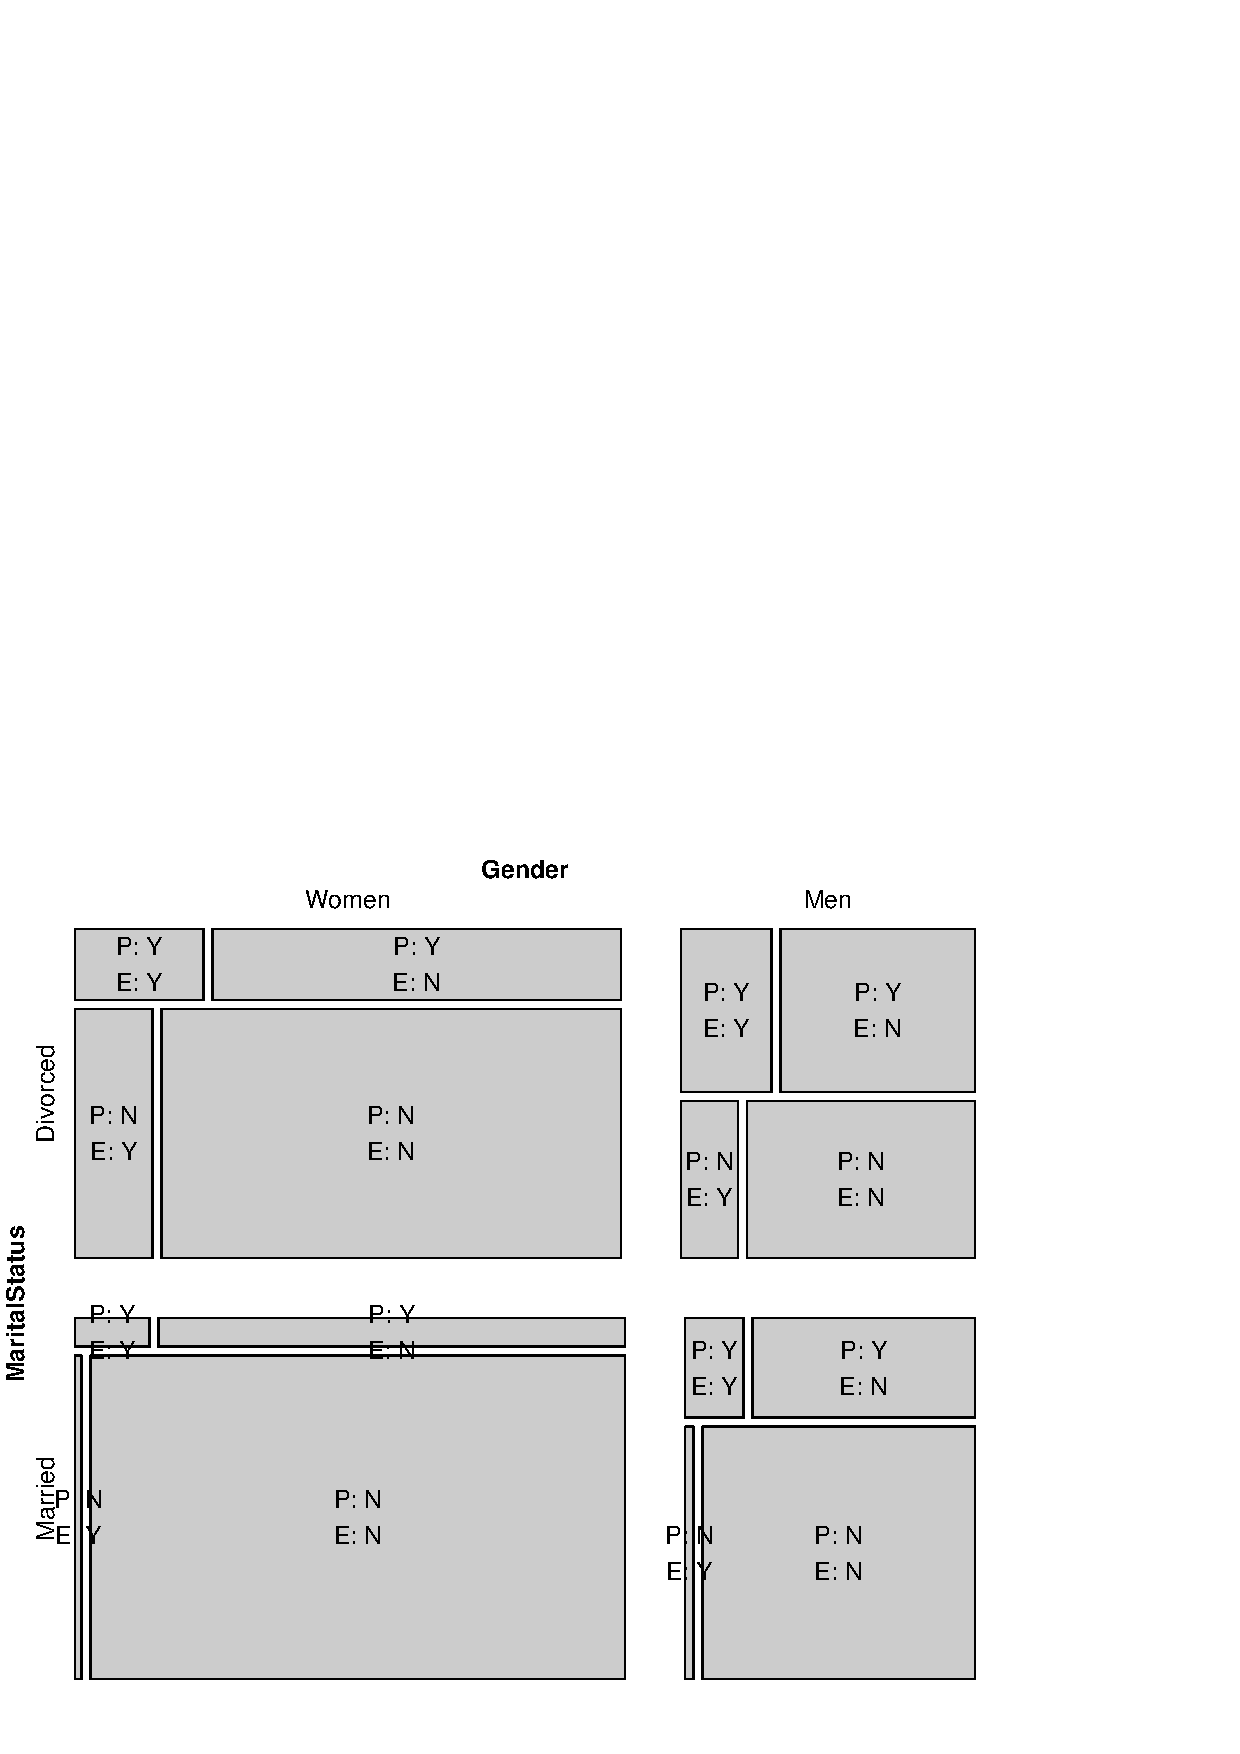
\includegraphics{labeling-conditionalfig}
\caption{Conditional labeling for the \data{PreSex}, labels abbreviated.}
\label{fig:conditional}
\end{center}
\end{figure}

\noindent Additionally, the cell labeling allows the user to add
arbitrary text to the cells by supplying a character array in the same
shape than the data array to the \code{text} argument (cells with missing values
are ignored). In the following example using the `Titanic' data, 
this is used to add all observed values greater
than 5 to the cells after the mosaic has been plotted (see Figure \ref{fig:text}):

\begin{Schunk}
\begin{Sinput}
> mosaic(Titanic, labeling_args = list(abbreviate = c(Survived = 1, 
+     Age = 4)), pop = FALSE)
> tab <- ifelse(Titanic < 6, NA, Titanic)
> labeling_cells(text = tab, clip = FALSE)(Titanic)
\end{Sinput}
\end{Schunk}

\begin{figure}[h]
\begin{center}
\includegraphics{labeling-textfig}
\caption{User-supplied Text added to a mosaic display of the \data{Titanic} data.}
\label{fig:text}
\end{center}
\end{figure}

\section{A simple list of labels: \texttt{labeling\_list()}}

If problems with overlapping labels cannot satisfactorily resolved,
the last remedy could be to simply list the levels below the plot
(see Figure \ref{fig:list}):

\begin{Schunk}
\begin{Sinput}
> mosaic(Titanic, labeling = labeling_list, margins = c(bottom = 5))
\end{Sinput}
\end{Schunk}

\setkeys{Gin}{width=0.8\textwidth}
\begin{figure}[h]
\begin{center}
\includegraphics{labeling-listfig}
\caption{Labels indicated below the plot.}
\label{fig:list}
\end{center}
\end{figure}

\noindent The number of columns can be specified.

\end{document}

